\begin{figure}[h]
	\centering

	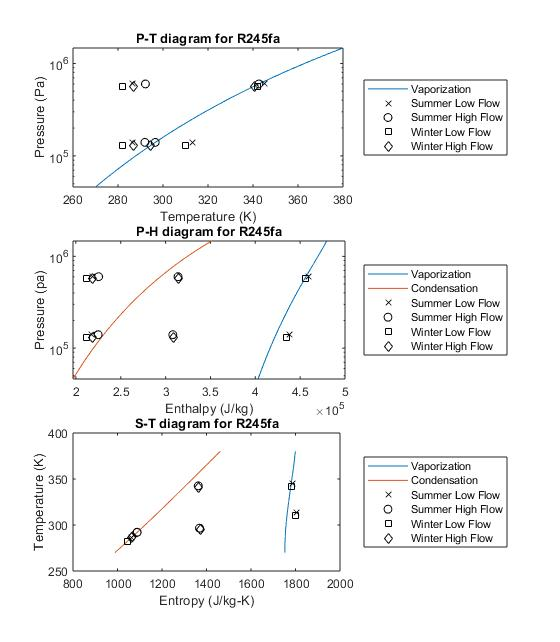
\includegraphics[width=\textwidth]{figures/GreenfieldThermoPlots}
	%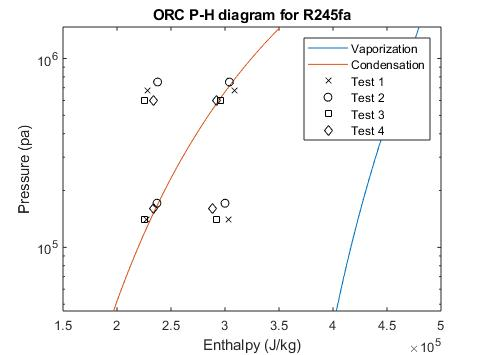
\includegraphics{figures/VerificationPH01}
	\caption{Thermodynamic plots of the simulated greenfield ORC prime power system plotting pressure against temperature (top), pressure against enthalpy (middle), and temperature against entropy (bottom). All points assume a source temperatures of \SI{364.5}{\kelvin} (\SI{91}{\degreeCelsius}), and source and sink flow rates of \SI{940}{\liter\per\minute}. Winter sink temperatures are assumed to be \SI{276.6}{\kelvin} (\SI{3.5}{\degreeCelsius}) while summer source temperatures are \SI{281.6}{\kelvin} (\SI{8.5}{\degreeCelsius}). High flow rate points have a working fluid mass flow rate of approximately \SI{8.4}{\kilogram\per\second}}
\label{fig:gf_themoplots}
\end{figure}